\chapter{叠}
\SourcePage{24}
我们将学习一些关于模空间和\Term{die}{叠}的知识，为讨论 Gromov–Witten 理论提供动机；希望还能涉及它的对数版本，以及 Donaldson–Thomas 理论。
总体任务，是使曲线计数具有确切含义，例如计算五次超曲面中亏格为零的全纯曲线的数目。这里有以下问题：
\begin{itemize}
\item 在经典计数代数几何中，要使计数成立，需要“一般位置论证”。横截性可能非常难以处理。
\item 可以将其转化为拓扑问题，例如 Grassmann 簇 $\operatorname{Gr}(k,n)$ 中的相交理论，也就是 Schubert 演算。
\item 一般来说，曲线空间，例如某个给定五次超曲面中的曲线空间，并不具有预期的维数。
\end{itemize}
\examnum{1}\begin{example}\label{ex:2.1}
考虑 Dwork 族 $f_\psi=0$。其中有 $375$ 条孤立直线，每条同构于 $\PP^1$，例如
$(u,v,-\zeta^ku,-\zeta^lv,0)$，其中 $[u:v]\in\PP^1$、$\zeta^5=1$、$0\le k,l\le4$；此外还有两个不可约的直线族。当次数大于 $1$ 时，总还会出现构成族的多重覆盖。
\end{example}
既然不能指望一般变形，我们该如何计数？解决办法是采用一种虚形式体系，这正是 Gromov–Witten 理论所做的事情。所得不变量在靶空间的族中保持不变。
\section{模空间}
我们关心一个由闭点组成的集合，具体说，是某些代数几何对象的同构类所构成的集合，例如簇或子簇的同构类。然后希望在它上面赋予额外结构。最理想的情形，是把它看作一个簇。对于参数概形 $T$ 及映射 $T\to M$，我们希望这样的映射对应于 $T$ 上的对象族。
\examnum{2}\begin{example}\label{ex:2.2}
固定 $N$。\Term{hilbertgaixing}{Hilbert 概形} $\operatorname{Hilb}(\PP^N)$ 用来分类闭子概形。具体而言，它具有如下泛性质：对于任意图表
\Eq{2.1}{\begin{tikzcd}Z\arrow[r,hook]\arrow[d,"{\text{平坦、固有}}"']\&T\times\PP^N\arrow[dl]\\T\end{tikzcd},}
\SourcePage{25}
存在唯一映射 $\varphi$，使
\Eq{2.2}{\begin{tikzcd}Z=\mathcal Z_T\arrow[r]\arrow[d]\&\mathcal Z\arrow[d]\\T\times\PP^N\arrow[r]\arrow[d]\&\operatorname{Hilb}(\PP^N)\times\PP^N\arrow[d]\\T\arrow[r,"{\varphi}"]\&\operatorname{Hilb}(\PP^N)\end{tikzcd}}
为相应的拉回图。从范畴论的角度看，这是说有一个反变函子
\Eq{2.3}{\begin{aligned}F:\Sch^{\mathrm{op}}&\longrightarrow\Set,\\T&\longmapsto\{\,Z\to T,\ Z\hookrightarrow T\times\PP^N\text{，且 }Z/T\text{ 平坦、固有}\,\},\end{aligned}}
由 $\operatorname{Hilb}(\PP^N)$ 表示。即存在自然同构
$F\simeq\Hom(\,\cdot\,,\operatorname{Hilb}(\PP^N))$。特别地，恒等态射
\[\id_{\operatorname{Hilb}(\PP^N)}\in\Hom(\operatorname{Hilb}(\PP^N),\operatorname{Hilb}(\PP^N))\]
对应于 $F(\operatorname{Hilb}(\PP^N))$ 中的对象，即万有族。
\end{example}
一个令人沮丧的观察是：对于曲线族，\footnote{对于任何对象可能带有自同构的其他模问题，也有同样的困难。}一般不能得到这样的可表性。
原因在于，存在所有纤维都同构、但整体不是乘积的曲线族。如果有上述表示对象，这样的族就会由一个常值分类映射拉回万有族，从而成为平凡族，产生矛盾。
\Lecture{6}{2019年9月17日}
\subsection{曲线的模问题}
我们大体沿着文献 \cite{ref9} 的思路展开。文献 \cite{ref8} 则是最早真正系统建立叠理论的工作。
我们希望对亏格为 $g$ 的完备曲线重复 Hilbert 概形的故事。
回忆族的概念。若 $S$ 是一个概形，可以把它想成某种参数空间，那么 $S$ 上一条亏格为 $g$ 的曲线，是一个态射 $\pi:C\to S$，满足：
\begin{enumerate}
\item $\pi$ 固有且平坦；
\item 对任意代数闭域 $K$ 及几何点 $\Spec K\to S$，几何纤维
\Eq{2.4}{C_s=\Spec K\times_SC}
位于图表
\Eq{2.5}{\begin{tikzcd}C_s\arrow[r]\arrow[d]\&C\arrow[d]\\\Spec K\arrow[r]\&S\end{tikzcd}}
中，并要求：
\begin{enumerate}
\item $C_s$ 约化、连通，且 $\dim C_s=1$；
\item $h^1(C_s,\OO_{C_s})=g$，即其算术亏格为 $g$。
\end{enumerate}
\end{enumerate}
还可以限制这些纤维允许出现的奇点，但目前我们不需要这样做。例如，可以要求 $C_s$ 非奇异。
\SourcePage{26}
现在遇到一个根本问题：函子
\Eq{2.6}{\begin{aligned}F_g:\Sch^{\mathrm{op}}&\longrightarrow\Set,\\S&\longmapsto\{\,X\to S\mid\text{亏格为 }g\text{ 的非奇异曲线族}\,\}/\simeq\end{aligned}}
不可表，因为存在非平凡的等平凡曲线族：$\pi:X\to S$ 只有在有限基变换后才变成平凡族。用反证法来看，假设它由某个 $M_g$ 表示，就有
\Eq{2.7}{\begin{tikzcd}T\times C_0\arrow[r]\arrow[d]\&X\arrow[r]\arrow[d]\&\mathcal C_g\arrow[d]\\T\arrow[r,"{\text{有限}}"']\arrow[rr,bend right=23,"{\text{常值}}"']\&S\arrow[r,"{\varphi}"]\&M_g\end{tikzcd}.}
复合映射为常值，将迫使 $\varphi$ 也是常值，与原来的族非平凡矛盾。
\examnum{3}\begin{example}\label{ex:2.3}
设 $C_0$ 是一条满足 $\Aut(C_0)\ne\{1\}$ 的曲线，例如一个二重覆盖 $C_0\to\PP^1$ 所给出的超椭圆曲线。具体例子是
\Eq{2.8}{y^2-(x-g-1)(x-g)\cdots(x-1)(x+1)\cdots(x+g+1)=0}
的射影闭包。有一个自同构交换两个分支，另一个自同构把 $x$ 映为 $-x$，因此有 $(\ZZ/2)^2$ 对称性。取一个满足 $\varphi^a=\id$ 的自同构 $\varphi$。回忆 $\mathbb G_m=\Spec\CC[x,x^{-1}]$。考虑 $(C_0\times\mathbb G_m)/(\ZZ/a)$。取一个本原 $a$ 次单位根 $\zeta\in\CC^\times$，作用为
\Eq{2.9}{(\varphi,\zeta):(z,t)\longmapsto(\varphi(z),\zeta t).}
这样得到一个 $\mathbb G_m$ 上的非平凡丛。
\end{example}
\begin{Note}{2.1}如果问题出在自同构上，为什么不只考虑没有自同构的曲线？事实上，限制到 $\Aut(C_s)=\{1\}$ 的曲线，确实可以使 $F_g$ 可表，但这种限制的用处并不大。\end{Note}
我们将改为把模空间构造成一个代数叠。这推广了概形的概念，并从一开始就把自同构纳入其中。
\section{叠}
另一个很好的参考资料是文献 \cite{ref20}，可惜它只有法文版本。\footnote{Siebert 教授说，这不是什么大问题，因为法语基本上就是英语。}
这里的想法，是形式化“由概形参数化的对象族，以及沿纤维的自同构”这一概念。
固定基概形 $S$，可将它想成 $\Spec\CC$。记 $\mathcal S=\Sch/S$，即 $S$ 上概形所构成的范畴。
\thmnum{definition}{1}\begin{definition}\label{def:2.1}
\begin{enumerate}
\item $\mathcal S$ 上的范畴，是一个范畴 $\mathcal F$ 连同函子 $p_{\mathcal F}:\mathcal F\to\mathcal S$。对于 $B\in\Obj(\mathcal S)$，有纤维范畴 $\mathcal F(B)$；它是 $\mathcal F$ 的子范畴，其对象为
\Eq{2.10}{\{\,X\in\Obj(\mathcal F)\mid p_{\mathcal F}(X)=B\,\},}
态射为
\Eq{2.11}{\{\,\varphi\in\Hom(\mathcal F)\mid p_{\mathcal F}(\varphi)=\id_B\,\}.}
\SourcePage{27}
\item 若满足以下条件，则 $\mathcal S$ 上的范畴称为 $\mathcal S$ 上的\Term{xianweiqunpai}{纤维群胚}：
\begin{enumerate}
\item 对每个 $\mathcal S$ 中的态射 $f:B'\to B$，以及 $B$ 上的对象 $X\in\Obj(\mathcal F)$，存在 $\mathcal F$ 中的态射 $\varphi:X'\to X$，使 $p_{\mathcal F}(\varphi)=f$：
\Eq{2.12}{\begin{tikzcd}X'\arrow[r,"{\varphi}"]\arrow[d]\&X\arrow[d,"{p_{\mathcal F}}"]\\B'\arrow[r,"{f}"]\&B\end{tikzcd}.}
\item 对任意满足 $p_{\mathcal F}(\varphi')=p_{\mathcal F}(\varphi'')\circ h$ 的图表，存在唯一 $\chi:X'\to X''$，覆盖 $h$，且 $\varphi'=\varphi''\circ\chi$：
\Eq{2.13}{\begin{tikzcd}X'\arrow[rr,"{\varphi'}",bend left]\arrow[r,dashed,"{\exists!\,\chi}"]\arrow[d]\&X''\arrow[r,"{\varphi''}"]\arrow[d]\&X\arrow[d,"{p_{\mathcal F}}"]\\B'\arrow[r,"{h}"]\arrow[rr,"{f'}",bend right]\&B''\arrow[r,"{f''}"]\&B\end{tikzcd}.}
\end{enumerate}
\end{enumerate}
\end{definition}
\begin{Note}{2.2}
\begin{enumerate}[label=(\roman*)]
\item 上述两条提升条件蕴含：$\varphi:X'\to X$ 是同构，当且仅当 $p_{\mathcal F}(\varphi)$ 是同构。
\item 若 $p_{\mathcal F}:\mathcal F\to\mathcal S$ 是纤维群胚，则每个 $\mathcal F(B)$ 都是群胚。
\item 唯一提升条件还说明，在
\Eq{2.14}{\begin{tikzcd}X'\arrow[r]\arrow[d]\&X\arrow[d]\\B'\arrow[r,"{f}"]\&B\end{tikzcd}}
中，$X'$ 在相差唯一同构的意义下唯一。记 $f^*X=X'$，称其为\Term{lahui}{拉回}。这一构造具有函子性：$\mathcal F(B)$ 中的态射 $\psi:X''\to X'$，给出典范态射 $f^*\psi:f^*X''\to f^*X'$。因此，$f:B'\to B$ 给出
\Eq{2.15}{f^*:\mathcal F(B)\longrightarrow\mathcal F(B').}
\end{enumerate}
\end{Note}
\examnum{4}\begin{example}[（可表函子）]\label{ex:2.4}
设 $F:\mathcal S^{\mathrm{op}}\to\Set$ 为反变函子。它给出一个纤维群胚：对象为 $(B,\beta)$，其中 $B\in\Obj(\mathcal S)$、$\beta\in F(B)$，投影为 $p_{\mathcal F}:(B,\beta)\mapsto B$。态射集合为
\Eq{2.16}{\Hom((B',\beta'),(B,\beta))=\{\,f:B'\to B\mid F(f)(\beta)=\beta'\,\}.}
例如，若 $X$ 是 $S$ 概形，则相应函子为 $F(B)=\Hom_S(B,X)$，且
\Eq{2.17}{F(\varphi:B'\to B):(f:B\to X)\longmapsto(f\circ\varphi:B'\to X).}
\SourcePage{28}
关联的群胚记为 $\underline X=\mathcal F$。它的对象是 $\mathcal S=\Sch/S$ 中的映射 $f:B\to X$，态射为交换三角形
\Eq{2.18}{\begin{tikzcd}B'\arrow[r,"{f'}"]\arrow[d,"{\varphi}"']\&X\\B\arrow[ur,"{f}"']\end{tikzcd},}
并有 $p_{\underline X}:(B\to X)\mapsto B$。
\end{example}
\examnum{5}\begin{example}[（商叠）]\label{ex:2.5}
设 $X/S$ 是带有平坦群概形 $G/S$ 作用的概形，例如 $G=\mathrm{GL}_n$。可以形成商 $[X/G]$。它的对象是图表
\Eq{2.19}{\begin{tikzcd}E\arrow[r,"{f}"]\arrow[d]\&X\\B\end{tikzcd},}
其中 $E/B$ 是 $G$ 主丛，$f$ 是 $G$ 等变态射。态射由下图给出：
\Eq{2.20}{\begin{tikzcd}E'\arrow[r]\arrow[rr,bend left]\arrow[d]\&E\arrow[r,"{f}"]\arrow[d]\&X\\B'\arrow[r]\&B\end{tikzcd},}
其中左侧方块必须是笛卡尔方块。
\end{example}
\begin{custom}{事实 1}\hypertarget{fact:1}{}\hypertarget{fact:2.1}{}
若 $G$ 在 $X$ 上自由作用，且商 $X/G$ 作为概形存在，则 $[X/G]\simeq X/G$。
\end{custom}
\examnum{6}\begin{example}[（$G$ 主丛的分类空间）]\label{ex:2.6}
当 $X=\mathrm{pt}$ 时，$BG=[\mathrm{pt}/G]$。
\end{example}
\Lecture{7}{2019年9月19日}
我们有三个主要例子。首先，若 $X$ 是概形，则得到
\Eq{2.21}{\underline X(S)=\Hom(S,X).}
这里把概形 $S$ 与其关联的纤维群胚联系起来。对于 $G$ 在 $X$ 上的作用，得到 $[X/G]$；对于函子 $F:(\Sch/S)^{\mathrm{op}}\to\Set$，得到 $S$ 上的纤维群胚 $\mathcal F$。
第三个例子是模群胚 $\mathcal M_g$。其对象是曲线族 $X\to B$，其中 $B$ 为任意概形，所有 $X_s$ 都非奇异；态射由笛卡尔图给出：
\Eq{2.22}{\begin{tikzcd}X'\arrow[r]\arrow[d]\&X\arrow[d]\\B'\arrow[r]\&B\end{tikzcd}.}
注意，它不是由同构类集合函子 $F_g$ 关联得到的群胚。
类似地，定义 $\mathcal M_g$ 上的万有曲线 $\mathcal C_g$。其对象为二元组 $(X\to B,\sigma)$，其中 $\sigma:B\to X$ 是截面。
\subsection{群胚的态射}
\thmnum{definition}{2}\begin{definition}\label{def:2.2}
$\mathcal S$ 上两个纤维群胚 $\mathcal F_1,\mathcal F_2$ 之间的态射，是一个函子 $p$，使
\Eq{2.23}{\begin{tikzcd}\mathcal F_1\arrow[r,"{p}"]\arrow[dr,"{p_{\mathcal F_1}}"']\&\mathcal F_2\arrow[d,"{p_{\mathcal F_2}}"]\\\&\mathcal S\end{tikzcd}}
交换，即 $p_{\mathcal F_1}=p_{\mathcal F_2}\circ p$。这里要求的是函子相等。
\end{definition}
\SourcePage{29}
\examnum{7}\begin{example}\label{ex:2.7}有遗忘函子 $\mathcal C_g\to\mathcal M_g$，它只是忘掉截面。\end{example}
\examnum{8}\begin{example}\label{ex:2.8}
概形态射 $f:X\to Y$，等价于关联群胚之间的态射 $p:\underline X\to\underline Y$。
\begin{proof}
“$\Rightarrow$”：在对象上，$p(B\xrightarrow{u}X)=(B\xrightarrow{f\circ u}Y)$；在态射上，
\Eq{2.24}{p\left(\begin{tikzcd}B\arrow[r,"{u}"]\&X\\B'\arrow[u,"{s}"]\arrow[ur,"{u'}"']\end{tikzcd}\right)=\left(\begin{tikzcd}B\arrow[r,"{f\circ u}"]\&Y\\B'\arrow[u,"{s}"]\arrow[ur,"{f\circ u'}"']\end{tikzcd}\right).}
“$\Leftarrow$”：若有
\Eq{2.25}{\begin{tikzcd}\underline X\arrow[r,"{p}"]\arrow[dr]\&\underline Y\arrow[d]\\\&\mathcal S\end{tikzcd},}
则 $p(X\xrightarrow{\id_X}X)=(X\xrightarrow fY)\in\Obj(\underline Y(X))$，其中 $f$ 是某个映射。这正是 Yoneda 引理的情形：$p$ 可以看作函子
\Eq{2.26}{\Hom_S(\,\cdot\,,X):\mathcal S^{\mathrm{op}}\longrightarrow\Set}
与另一个函子 $G:\mathcal S^{\mathrm{op}}\to\Set$ 之间的自然变换。Yoneda 引理给出
\Eq{2.27}{\operatorname{Nat}(\Hom_S(\,\cdot\,,X),G)\xrightarrow{\sim}G(X),\qquad\Phi\longmapsto\Phi(\id_X).}
这说明 $p$ 由 $f$ 诱导。
\end{proof}
\end{example}
\examnum{9}\begin{example}\label{ex:2.9}
类似地，对于概形 $B$ 及 $\mathcal S$ 上的纤维群胚 $\mathcal F$，有范畴等价
\Eq{2.28}{\Hom_{\mathcal S}(\underline B,\mathcal F)\simeq\mathcal F(B),\qquad p\longmapsto p(\id_B).}
\end{example}
\examnum{10}\begin{example}\label{ex:2.10}
基概形 $S$ 对应于其关联群胚 $\underline S$。对于 $\mathcal S$ 上任意纤维群胚 $\mathcal F$，可以把 $p_{\mathcal F}:\mathcal F\to\mathcal S$ 看成群胚态射 $\mathcal F\to\underline S$。
\end{example}
\examnum{11}\begin{example}\label{ex:2.11}
设 $X/S$ 为概形，$G/S$ 为作用于它的群概形。这给出商态射 $q:X\to[X/G]$。在对象上，
\Eq{2.29}{(B\xrightarrow sX)\longmapsto\left(\begin{tikzcd}G\times B\arrow[r,"{(g,b)\mapsto g\cdot s(b)}"]\arrow[d]\&X\\B\end{tikzcd}\right),}
其中 $G$ 在 $G\times B$ 上作用。
\SourcePage{30}
在态射上，
\Eq{2.30}{\left(\begin{tikzcd}B'\arrow[r,"{f}"]\arrow[dr,"{s'}"']\&B\arrow[d,"{s}"]\\\&X\end{tikzcd}\right)\longmapsto\left(\begin{tikzcd}G\times B'\arrow[r,"{\id\times f}"]\arrow[rr,bend left]\arrow[d]\&G\times B\arrow[r]\arrow[d]\&X\\B'\arrow[r,"{f}"]\&B\end{tikzcd}\right).}
\end{example}
\begin{Note}{2.3}群胚的同构由 $\mathcal S$ 上的范畴等价给出。特别地，$p:\mathcal F_1\xrightarrow{\sim}\mathcal F_2$ 未必有严格逆函子，只需有拟逆 $q:\mathcal F_2\to\mathcal F_1$，使 $pq$ 自然同构于 $\id_{\mathcal F_2}$，而 $qp$ 自然同构于 $\id_{\mathcal F_1}$。\end{Note}
$\mathcal S$ 上的纤维群胚实际上构成一个 $2$ 范畴 $\operatorname{Grpd}/\mathcal S$。对象是 $\mathcal S$ 上的群胚，$1$ 态射是它们之间位于 $\mathcal S$ 上的函子；现在还存在另一类态射，称为 $2$ 态射，也就是态射之间的态射。
\begin{Note}{2.4}若不讨论这些 $2$ 态射，我们甚至无法定义笛卡尔图。因此，确实必须理解它们。\end{Note}
\thmnum{proposition}{1}\begin{proposition}\label{pro:2.1}
设 $X,Y$ 是概形。则 $X\simeq Y$ 作为概形成立，当且仅当 $\underline X\simeq\underline Y$ 作为 $\mathcal S$ 上的群胚成立。
\end{proposition}
\begin{proof}
“$\Rightarrow$”：设 $f:X\to Y$ 是同构，则诱导映射 $p:\underline X\to\underline Y$ 是严格等价。事实上，$f^{-1}$ 诱导 $q:\underline Y\to\underline X$，满足 $pq=\id_{\underline Y}$、$qp=\id_{\underline X}$。
“$\Leftarrow$”：设 $p$ 为等价，$q$ 为拟逆。已经看到，$p,q$ 分别由 $f:X\to Y$ 与 $g:Y\to X$ 诱导。因此
$qp(X\xrightarrow{\id_X}X)=(X\xrightarrow{gf}X)$，作为 $\underline X$ 中的对象。由于 $q$ 是 $p$ 的拟逆，存在图表中的同构
\Eq{2.31}{\begin{tikzcd}X\arrow[r,"{\simeq}"]\arrow[dr,"{gf}"']\&X\arrow[d,"{\id_X}"]\\\&X\end{tikzcd},}
且该同构位于 $\id_X$ 上，所以 $gf=\id_X$。对 $fg$ 同理，因而 $f$ 是同构。
\end{proof}
\begin{Note}{2.5}这说明，在纤维群胚的范畴中包含着概形范畴。今后常直接写 $X$，而不再区分 $X$ 与 $\underline X$。同样，也会根据语境用 $S$ 表示基概形、相应的概形范畴或关联群胚。\end{Note}
\subsection{纤维积与笛卡尔图}
\thmnum{definition}{3}\begin{definition}\label{def:2.3}
考虑 $\mathcal S$ 上三个纤维群胚 $\mathcal F,\mathcal G,\mathcal H$，及态射 $f:\mathcal F\to\mathcal G$、$h:\mathcal H\to\mathcal G$。其\Term{xianweiji}{纤维积}定义如下。位于基 $B$ 上的对象，是三元组 $(x,y,\psi)$，其中 $x\in\mathcal F(B)$、$y\in\mathcal H(B)$，而 $\psi:f(x)\to h(y)$ 是 $\mathcal G(B)$ 中的同构。位于 $B$ 上、从 $(x',y',\psi')$ 到 $(x,y,\psi)$ 的态射是一对
\Eq{2.32}{(x'\xrightarrow\alpha x,\ y'\xrightarrow\beta y),}
满足
\Eq{2.33}{\psi\circ f(\alpha)=h(\beta)\circ\psi'.}
\end{definition}
\SourcePage{31}
于是有图表
\Eq{2.34}{\begin{tikzcd}\mathcal F\times_{\mathcal G}\mathcal H\arrow[r,"{q}"]\arrow[d,"{p}"']\&\mathcal H\arrow[d,"{h}"]\\\mathcal F\arrow[r,"{f}"]\&\mathcal G\end{tikzcd},}
它只在相差一个 $2$ 态射的意义下交换。
\begin{Warning}{2.1}这一图表一般并不严格交换，因为
\Eq{2.35}{fp(x,y,\psi)=f(x),\qquad hq(x,y,\psi)=h(y).}
但函子之间存在自然同构 $fp\simeq hq$，即 \eqref{eq:2.34} 是 $2$ 交换的。因此，需要 $\psi$ 所给出的扭合，才使两者相容。
\end{Warning}
$\mathcal F\times_{\mathcal G}\mathcal H$ 对 $2$ 交换图具有泛性质：
\Eq{2.36}{\begin{tikzcd}\mathcal T\arrow[drr,bend left]\arrow[ddr,bend right]\arrow[dr,dashed,"{\exists!}" description]\\\&\mathcal F\times_{\mathcal G}\mathcal H\arrow[r]\arrow[d]\&\mathcal H\arrow[d]\\\&\mathcal F\arrow[r]\&\mathcal G\end{tikzcd}.}
\examnum{12}\begin{example}\label{ex:2.12}对于概形 $X,Y,Z$，有
\Eq{2.37}{\underline{X\times_ZY}\simeq\underline X\times_{\underline Z}\underline Y.}
\end{example}
\examnum{13}\begin{example}[（基变换）]\label{ex:2.13}
若 $T\to S$ 是概形态射，则 $T\times_S\mathcal F$ 是 $T$ 上的纤维群胚。事实上，对于任意 $B\to T$，$\mathcal F(B)$ 与 $(T\times_S\mathcal F)(B)$ 等价，其对象具有图表
\Eq{2.38}{\begin{tikzcd}X\arrow[d]\\B\arrow[r]\arrow[dr]\&T\arrow[d]\\\&S\end{tikzcd}\qquad X\in\mathcal F(B).}
\end{example}
\subsection{叠的定义}
我们希望更接近一种可以在其中做代数几何的对象。
\thmnum{definition}{4}\begin{definition}[同构函子]\label{def:2.4}
设 $(\mathcal F,p_{\mathcal F})$ 是 $\mathcal S$ 上的纤维群胚，$B$ 是 $S$ 上的概形，$X,Y\in\Obj(\mathcal F(B))$。定义反变函子
\Eq{2.39}{\operatorname{Iso}_B(X,Y):(\Sch/B)^{\mathrm{op}}\longrightarrow\Set.}
在对象上，它将
\Eq{2.40}{(B'\xrightarrow fB)\longmapsto\{\,f^*X\xrightarrow\varphi f^*Y\mid\varphi\text{ 是同构}\,\}.}
在态射上，对于 $g=f\circ h$，有
\Eq{2.41}{\begin{tikzcd}B''\arrow[r,"{h}"]\arrow[dr,"{g}"']\&B'\arrow[d,"{f}"]\\\&B\end{tikzcd}\quad\longmapsto\quad\bigl[(f^*X\to f^*Y)\mapsto(h^*f^*X\to h^*f^*Y)\bigr],}
其中 $h^*f^*X\simeq g^*X$，$h^*f^*Y\simeq g^*Y$。
\end{definition}
\SourcePage{32}
\thmnum{theorem}{2}\begin{theorem}[Deligne–Mumford]\label{thm:2.2}
设 $X/B,Y/B$ 是亏格为 $2$ 的曲线族，则同构函子 $\operatorname{Iso}_B(X,Y)$ 由一个概形表示。
\end{theorem}
\begin{proof}
我们有相对典范线丛 $\omega_{X/B}$ 和 $\omega_{Y/B}$。它们相对丰，因此其足够高次幂给出 $B$ 上的射影空间嵌入。这些是典范丛，故对任意 $f:B'\to B$，任一同构 $f^*X\to f^*Y$ 都保持这一极化。现在，可以对同构的图像使用相对 Hilbert 概形。
\end{proof}
\begin{Note}{2.6}$\operatorname{Iso}_B(X,Y)$ 在 $B$ 上有限且非分歧，但一般并不平坦，例如纤维的基数可能跳跃。\end{Note}
\Lecture{8}{2019年9月24日}
\thmnum{definition}{5}\begin{definition}[叠]\label{def:2.5}
$\mathcal S$ 上的纤维群胚 $(\mathcal F,p_{\mathcal F})$ 称为叠，如果：
\begin{enumerate}
\item 对 $S$ 上任意 $B$ 及 $X,X'\in\Obj(\mathcal F(B))$，$\operatorname{Iso}_B(X,X')$ 是平展拓扑中的层；
\item 对 $B$ 的平展覆盖 $\{B_i\to B\}$、对象 $X_i\in\Obj(\mathcal F(B_i))$，以及满足余循环条件的同构
\Eq{2.42}{\varphi_{ij}:X_j|_{B_i\times_BB_j}\longrightarrow X_i|_{B_i\times_BB_j},}
这些对象能够粘合：存在 $X\in\Obj(\mathcal F(B))$ 和同构 $X|_{B_i}\simeq X_i$，并诱导给定的 $\varphi_{ij}$。
\end{enumerate}
\end{definition}
\begin{Note}{2.7}第一个条件可理解为态射的下降，第二个条件可理解为对象的下降。\end{Note}
\UnnumberedSubsection{平展拓扑}
关于这一主题，权威参考资料是文献 \cite{ref18}，而文献 \cite{ref23} 更容易阅读。用\Term{pingzhan}{平展态射} $U\to X$ 替代 Zariski 开子集。直观上，可以把它理解为非分歧、局部像微分同胚的映射。$U\to X$ 与 $V\to X$ 的“交”，由 $U\times_XV\to X$ 给出。这是所谓 Grothendieck 拓扑的一个例子。
形式上，光滑、非分歧和平展态射 $f:X\to Y$ 都是概形之间的有限型态射。设 $T=\Spec A\hookrightarrow T'=\Spec A'$ 是一个无穷小扩张，即 $A=A'/I$，且某个 $n$ 满足 $I^n=0$。
\examnum{14}\begin{example}\label{ex:2.14}
可考虑 $\Spec k\hookrightarrow\Spec k[\epsilon]/(\epsilon^n)$，以及相邻阶的无穷小加厚
$\Spec k[\epsilon]/(\epsilon^n)\hookrightarrow\Spec k[\epsilon]/(\epsilon^{n+1})$。当 $n=2$ 时，$\Spec k\hookrightarrow\Spec k[\epsilon]/(\epsilon^2)$ 是平方零扩张。
\end{example}
在这一情形下，考察所有图表
\Eq{2.43}{\begin{tikzcd}[row sep=2.5em,column sep=3em]T\arrow[r,"{\varphi}"]\arrow[d,hook]\&X\arrow[d,"{f}"]\\T'\arrow[r,"{\psi}"']\arrow[ur,dashed,"{\exists\widetilde\psi?}"]\&Y\end{tikzcd}.}
然后询问两个性质：提升 $\widetilde\psi$ 是否存在，以及它是否唯一。
\Needspace{7\baselineskip}\thmnum{definition}{6}\begin{definition}\label{def:2.6}
称 $f$ 形式上：
\begin{enumerate}
\item 光滑，当且仅当这样的提升局部存在；
\item 非分歧，当且仅当这样的提升至多唯一；
\item 平展，当且仅当这样的提升存在且唯一。
\end{enumerate}
\end{definition}
\examnum{15}\begin{example}\label{ex:2.15}
图 \ref{fig:2.1} 中的二重覆盖是平展的，但图中的曲线本身并不光滑。
\end{example}
\SourcePage{33}
\begin{figure}[H]\centering
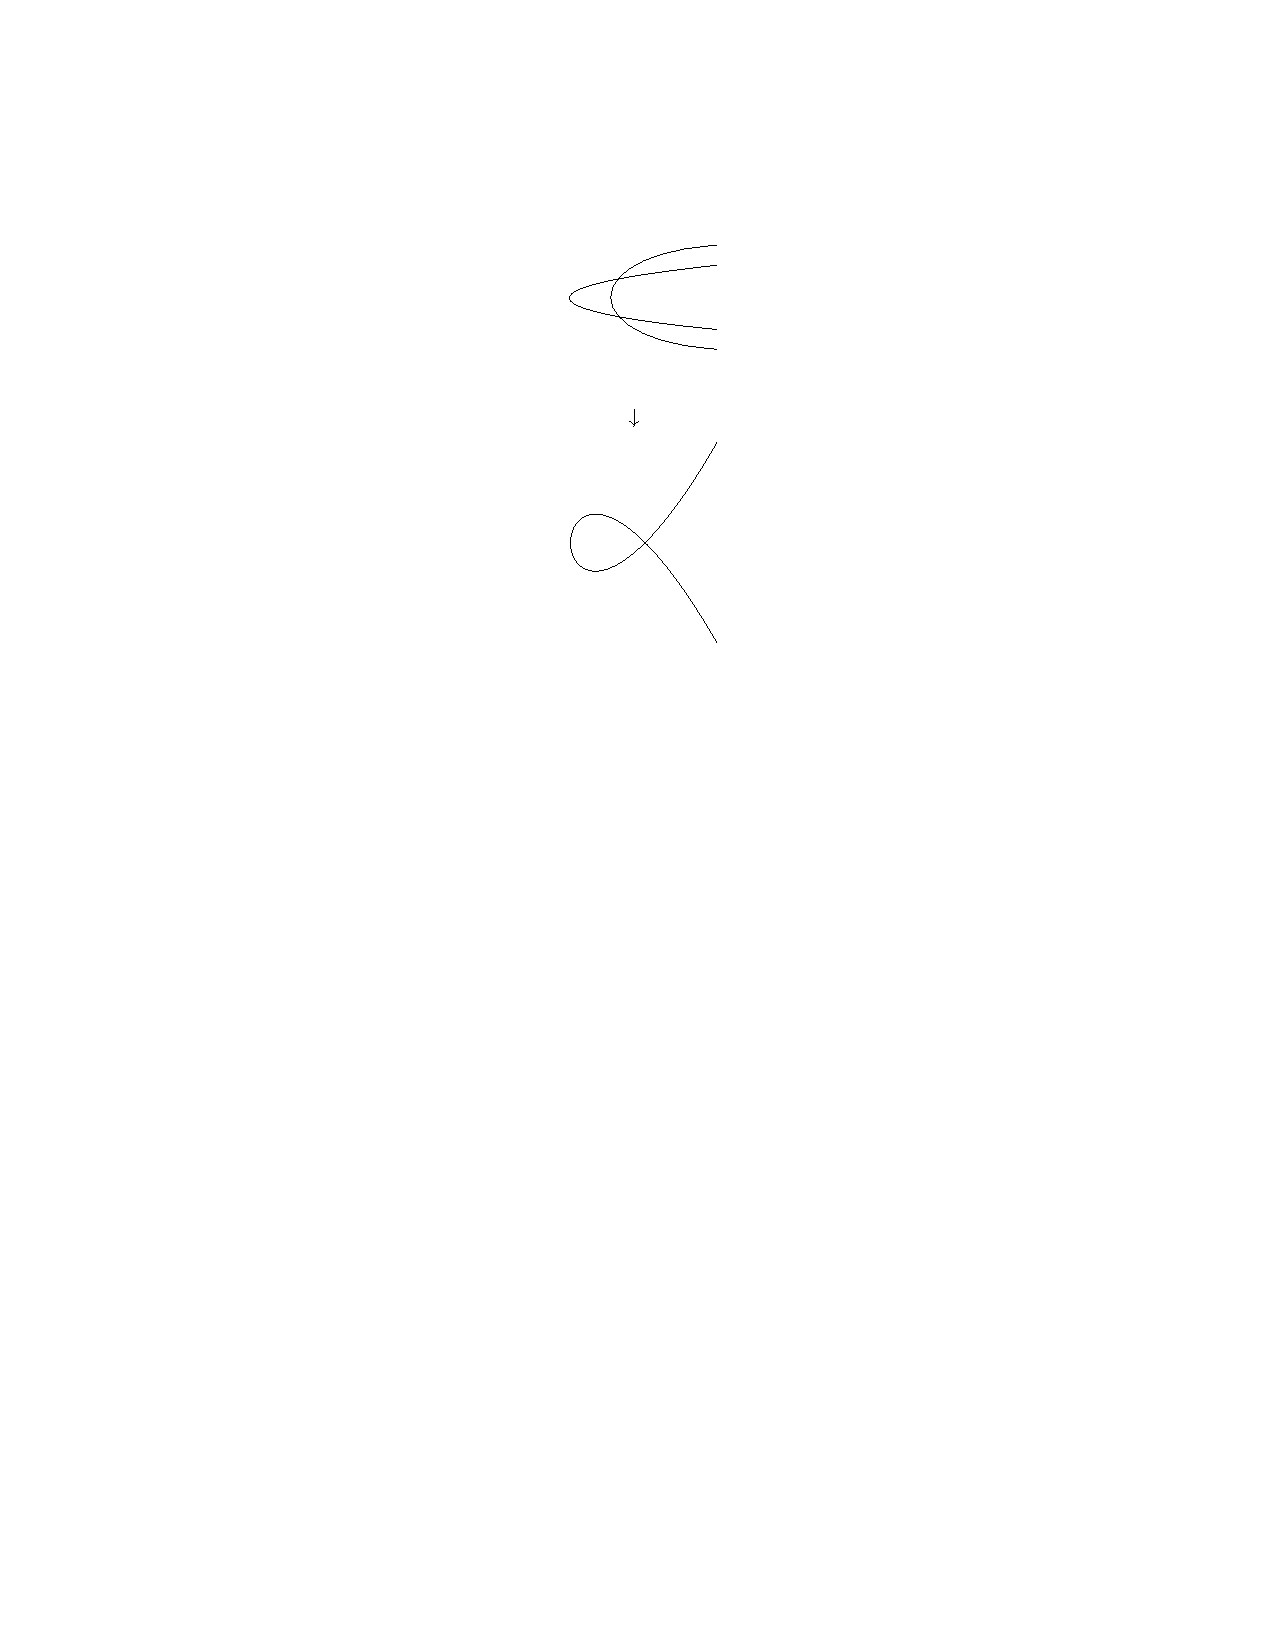
\includegraphics[width=0.4798\linewidth]{images/fig-2-1.pdf}
\caption{曲线 $V(y^2-x^3-x^2)$ 的二重覆盖。}\label{fig:2.1}
\end{figure}
光滑情形应当像一个投影：切向量可以提升，但提升未必唯一。平展情形则像把两条曲线映到一条曲线上；通过 $\varphi$ 选定上方的一点后，提升就是唯一的。一个有分歧且并非光滑的例子，是代数映射 $z\mapsto z^2$ 所给出的覆盖 $\mathbb A^1\to\mathbb A^1$。在分歧点，非零切向量不能提升，零切向量则可以有不唯一的提升。
\subsection{叠的例子}
\examnum{16}\begin{example}\label{ex:2.16}
设 $\mathcal F$ 是由函子
\Eq{2.44}{F:\mathcal S^{\mathrm{op}}\longrightarrow\Set}
关联得到的纤维群胚。则 $\mathcal F$ 是叠，当且仅当 $F$ 是平展拓扑中的集合层。若 $F=\Hom_S(-,X)$，$X\in\mathcal S$，则它是叠，这需要态射的平展下降。注意，模函子 $F_g$ 一般不是层，因此其关联群胚不是叠：曲线族的同构类未必能满足层的粘合要求。
\end{example}
\examnum{17}\begin{example}\label{ex:2.17}模群胚 $\mathcal M_g$ 是叠。\end{example}
\thmnum{proposition}{3}\begin{proposition}\label{pro:2.3}
设 $G/S$ 是一个平坦群概形，采用仿射、分离的情形，且 $G$ 作用于 $X$。则 $[X/G]$ 是叠。
\end{proposition}
\begin{proof}
对于对象下降条件，需要 $G$ 主丛，即 $G$ 挠子的平展下降。
对于态射下降条件，我们断言 $\operatorname{Iso}_B(f,f')$ 可由概形表示，其中对象为
\Eq{2.45}{\begin{tikzcd}E\arrow[r,"{f}"]\arrow[d]\&X\&E'\arrow[l,"{f'}"']\arrow[dll]\\B\end{tikzcd}.}
可以在使主丛平凡的平展局部计算，并用下降得到结论。因此暂设 $E=B\times G=E'$。选取截面 $\sigma:B\to E$ 和 $\sigma':B\to E'$，得到两个态射 $s=f\circ\sigma$、$s'=f'\circ\sigma':B\to X$。
\SourcePage{34}
主丛之间的等变同构由一个 $G$ 值参数描述；与 $f,f'$ 相容，要求 $s=g\cdot s'$。所以
\Eq{2.46}{\operatorname{Iso}_B(f,f')\simeq B\times_{X\times_SX}(G\times_SX),}
其中 $G\times_SX\to X\times_SX$ 把 $(g,x)$ 映为 $(g\cdot x,x)$。它位于纤维图
\Eq{2.47}{\begin{tikzcd}\operatorname{Iso}_B(f,f')\arrow[r]\arrow[d]\&G\times_SX\arrow[d,"{(g,x)\mapsto(gx,x)}"]\\B\arrow[r,"{(s,s')}"]\&X\times_SX\end{tikzcd}.}

\end{proof}
\begin{Note}{2.8}对概形本身，而不仅是其态射，进行平展下降，会导向代数空间的概念；这是 Artin 与 Knutson 的工作。\end{Note}
\examnum{18}\begin{example}\label{ex:2.18}
若 $\mathcal F,\mathcal G,\mathcal H$ 都是叠，且有态射 $\mathcal F\to\mathcal G$ 和 $\mathcal H\to\mathcal G$，则 $\mathcal F\times_{\mathcal G}\mathcal H$ 也是叠。
\end{example}
\subsection{可表态射}
某些叠之间的态射具有类似于概形的性质。
\thmnum{definition}{7}\begin{definition}\label{def:2.7}
叠态射 $f:\mathcal F\to\mathcal G$ 称为\Term{kebiaotaishi}{可表态射}，如果对任意概形 $B$ 及态射 $B\to\mathcal G$，纤维积 $B\times_{\mathcal G}\mathcal F$ 是一个概形的关联群胚。更一般且更合适的定义，允许它是代数空间。
\end{definition}
\examnum{19}\begin{example}\label{ex:2.19}
考虑 $X\to[X/G]$。使下图成为纤维图的 $E$ 是一个概形：
\Eq{2.48}{\begin{tikzcd}E\arrow[r]\arrow[d]\&X\arrow[d]\\B\arrow[r]\&{[X/G]}\end{tikzcd}.}
\end{example}
\examnum{20}\begin{example}\label{ex:2.20}
回忆，$\mathcal M_g$ 是亏格为 $g$ 的光滑曲线的模叠，而 $\mathcal C_g\to\mathcal M_g$ 还记住一个截面。对于 $B$ 上的曲线族 $C$，有纤维图
\Eq{2.49}{\begin{tikzcd}C\arrow[r]\arrow[d]\&\mathcal C_g\arrow[d]\\B\arrow[r]\&\mathcal M_g\end{tikzcd}.}
\end{example}
其思想是：对于在基变换下稳定的概形态射性质，它们与叠的思想相容，因此可以把这些性质移到叠的世界中。
\thmnum{definition}{8}\begin{definition}\label{def:2.8}
设 $\mathcal F\to\mathcal G$ 可表。对于在基变换下稳定的概形态射性质 $P$，\footnote{例如有限型、分离、平坦、仿射、固有等。}称该态射具有性质 $P$，如果对于每个概形 $B$ 及态射 $B\to\mathcal G$，$B\times_{\mathcal G}\mathcal F\to B$ 都具有该性质。
\end{definition}
\examnum{21}\begin{example}\label{ex:2.21}
若 $G/S$ 光滑，且 $G$ 作用于 $X$，则 $X\to[X/G]$ 光滑。
\end{example}
\SourcePage{35}
\subsection{Deligne–Mumford 叠的定义}
\thmnum{definition}{9}\begin{definition}\label{def:2.9}
叠 $\mathcal F$ 称为 \Term{delignemumforddie}{Deligne–Mumford 叠}，如果：
\begin{enumerate}
\item 对角态射 $\Delta_{\mathcal F}:\mathcal F\to\mathcal F\times_S\mathcal F$ 可表、拟紧且分离。\footnote{后两个条件有时会被放宽。}若 $\Delta_{\mathcal F}$ 还固有，则称 $\mathcal F$ 分离。
\item 存在平展满射 $\varphi:U\to\mathcal F$，其中 $U$ 是概形，称为平展图册。
\end{enumerate}
\end{definition}
\Lecture{9}{2019年9月26日}
下面作一些说明。
\begin{enumerate}
\item 首先讨论 $\Delta_{\mathcal X}$ 的可表性。
\thmnum{proposition}{4}\begin{proposition}\label{pro:2.4}
$\Delta_{\mathcal X}$ 可表，当且仅当每个从概形 $B$ 到 $\mathcal X$ 的态射都可表。
\end{proposition}
\begin{proof}
“$\Rightarrow$”：对于两个概形 $B,B'$，要证明图表中的 $B'\times_{\mathcal X}B$ 是概形：
\Eq{2.50}{\begin{tikzcd}B'\times_{\mathcal X}B\arrow[r]\arrow[d]\&B\arrow[d,"{f}"]\\B'\arrow[r,"{g}"]\&\mathcal X\end{tikzcd}.}
这由 $\Delta_{\mathcal X}$ 可表推出，因为有纤维图
\Eq{2.51}{\begin{tikzcd}B'\times_{\mathcal X}B\arrow[r]\arrow[d]\&\mathcal X\arrow[d,"{\Delta_{\mathcal X}}"]\\B'\times_SB\arrow[r,"{g\times f}"]\&\mathcal X\times_S\mathcal X\end{tikzcd}.}

\end{proof}
另一个方面是：若 $X,Y\in\Obj(\mathcal F(B))$，则 $\operatorname{Iso}_B(X,Y)$ 由概形表示。
\begin{proof}
$X,Y$ 对应于两个映射 $f,g:B\to\mathcal X$。同构函子由下面的纤维积表示：
\Eq{2.52}{\begin{tikzcd}B\times_{\mathcal X\times_S\mathcal X}\mathcal X\arrow[r]\arrow[d]\&\mathcal X\arrow[d,"{\Delta_{\mathcal X}}"]\\B\arrow[r,"{(f,g)}"]\&\mathcal X\times_S\mathcal X\end{tikzcd}.}
由可表性，它就是一个概形。
\end{proof}
\item $\Delta_{\mathcal X}$ 拟紧：我们不希望 $\operatorname{Iso}_B(X,Y)$ 过于失控。这个条件可以放宽，例如 Stacks Project 采用的定义就更一般。
\item $\Delta_{\mathcal X}$ 分离：若一个同构在一般点处为恒等，它就为恒等。
\item 什么时候 $\Delta_{\mathcal X}$ 固有？这应当与叠 $\mathcal X$ 的分离性有关。对于概形，通常要求 $X\to X\times_SX$ 是闭嵌入。
\SourcePage{36}
\item 图册提供了 Artin 环上的变形所需的通用变形空间。写 $\bar A=A/I$，其中 $I^n=0$。其想法是：在
\Eq{2.53}{\begin{tikzcd}\Spec\bar A\arrow[r]\arrow[d]\&U\arrow[d]\\\Spec A\arrow[r]\arrow[ur,dashed]\&\mathcal X\end{tikzcd}}
中得到相应的唯一提升。
\item 图册平展，使 $\Delta_{\mathcal F}$ 非分歧，即自同构在某种意义上是离散的。若只有光滑图册，则称为 Artin 叠，或代数叠。
\examnum{22}\begin{example}\label{ex:2.22}
对于平坦但未必平展的群概形 $G/S$，相应的 $BG=[\mathrm{pt}/G]$ 给出 Artin 叠的例子。
\end{example}
\end{enumerate}
\UnnumberedSubsection{叠的分离性}
\thmnum{lemma}{5}\begin{lemma}\label{lem:2.5}
设 $f:\mathcal F\to\mathcal G$ 是满足上述对角态射条件的叠之间的态射，则相对对角态射 $\Delta_{\mathcal F/\mathcal G}:\mathcal F\to\mathcal F\times_{\mathcal G}\mathcal F$ 可表。
\end{lemma}
\begin{proof}见文献 \cite{ref20}。\end{proof}
\UnnumberedSubsection{Artin 叠成为 Deligne–Mumford 叠的判别准则}
\thmnum{theorem}{6}\begin{theorem}\label{thm:2.6}
设 $\mathcal F$ 为 Noether 概形 $S$ 上的代数叠，具有一个在 $S$ 上有限型的光滑图册 $U\to\mathcal F$。则 $\mathcal F$ 是 Deligne–Mumford 叠，当且仅当 $\Delta_{\mathcal F}$ 非分歧。
\end{theorem}
\begin{proof}见文献 \cite{ref20}，或文献 \cite{ref9} 的定理 2.1。\end{proof}
\thmnum{corollary}{7}\begin{corollary}\label{cor:2.7}
设 $G/S$ 为作用于 Noether 概形 $X/S$ 的光滑仿射群概形，两者在 $S$ 上均有限型，且几何点的稳定子有限并约化。则：
\begin{enumerate}[label=(\roman*)]
\item $[X/G]$ 是 Deligne–Mumford 叠；若稳定子平凡，它是代数空间。
\item $[X/G]$ 分离，当且仅当作用态射固有。
\end{enumerate}
\end{corollary}
\begin{proof}
证明第一点。稳定子有限并约化意味着，对于任意对象
\Eq{2.54}{B\to[X/G]\quad\longleftrightarrow\quad\left(\begin{tikzcd}E\arrow[r]\arrow[d]\&X\\B\end{tikzcd}\right),}
$\operatorname{Iso}_B(E,E)\to B$ 非分歧。因此 $\Delta_{[X/G]}$ 非分歧，而 $X\to[X/G]$ 光滑，由\hyperref[thm:2.6]{上述定理}可知 $[X/G]$ 是 Deligne–Mumford 叠。
\end{proof}
\section{稳定曲线}
要得到曲线的完备模叠，即直观上的紧模叠，必须加入奇异曲线。Deligne 与 Mumford 的洞见是：加入结点就足够了。\footnote{结点的意思是，平展局部看起来像 $V(zw)\subset\mathbb A^2$。}
\SourcePage{37}
\Needspace{10\baselineskip}\thmnum{definition}{10}\begin{definition}\label{def:2.10}
概形 $S$ 上的一条 Deligne–Mumford 稳定曲线，是固有平坦态射 $\pi:C\to S$，满足：
\begin{enumerate}[label=(\roman*)]
\item 几何纤维 $C_s$ 约化、连通、一维，其奇点至多为结点；
\item 若 $E\subset C_s$ 是一个正规化为光滑有理曲线的不可约分支，$\nu:\widetilde E\to E$ 为正规化，则奇点在 $\widetilde E$ 中的原像至少有 $3$ 个。
\end{enumerate}
同时，不允许 $C_s$ 是亏格为 $0$ 或 $1$ 的光滑曲线。
\end{definition}
\begin{Note}{2.9}条件 (ii) 连同上述排除情形，等价于 $\Aut(C_s)$ 有限。\end{Note}
注意，亏格为 $g=h^1(C_s,\OO_{C_s})$。这些对象立即构成亏格为 $g$ 的稳定曲线群胚 $\overline{\mathcal M}_g$；目前，它是 $\ZZ$ 上的一个叠。
\subsection{稳定曲线模叠是 Deligne–Mumford 叠}
回忆，对于稳定曲线，$\pi:C\to S$ 是平展局部完全交态射，因此具有相对对偶化可逆层 $\omega_{C/S}$。在几何纤维上，可显式考虑正规化
\Eq{2.55}{\nu:C_s'\longrightarrow C_s,\qquad x_i,y_i\longmapsto\text{第 }i\text{ 个结点}.}
于是
\Eq{2.56}{\nu^*\omega_{C_s}=\omega_{C_s'}(x_1+\cdots+x_r+y_1+\cdots+y_r).}
若 $\alpha\in\omega_{C_s}(U)$，其中 $U$ 为第 $i$ 个结点的邻域，则 $\nu^*\alpha$ 是一个有理一形式，且
\Eq{2.57}{\operatorname{Res}_{x_i}(\nu^*\alpha)+\operatorname{Res}_{y_i}(\nu^*\alpha)=0.}
现在用 $\omega_{C/S}^{\otimes n}$ 将 $C/S$ 嵌入某个 $\PP_S^N$。
\thmnum{theorem}{8}\begin{theorem}\label{thm:2.8}
若 $g\ge2$，则当 $n\ge3$ 时，$\omega_{C/S}^{\otimes n}$ 相对甚丰。此外，$\pi_*(\omega_{C/S}^{\otimes n})$ 局部自由，秩为 $(2n-1)(g-1)$。
\end{theorem}
\Lecture{10}{2019年10月1日}
\begin{proof}
这里只给出证明概要。对于光滑曲线，当 $g\ge3$ 时，$\omega_{C/S}^{\otimes n}$ 在 $n\ge2$ 时就相对甚丰；亏格 $2$ 时采用 $n\ge3$。先考虑 $S=\Spec k$。由 Riemann–Roch 定理与 Serre 对偶性，
\Eq{2.58}{h^0(C,\omega_C^{\otimes n})=h^1(C,\omega_C^{\otimes n})+\deg(\omega_C^{\otimes n})+1-g,}
\Eq{2.59}{=h^0\bigl(C,(\omega_C^{\otimes n})^{-1}\otimes\omega_C\bigr)+n(2g-2)+1-g.}
对于光滑曲线，$(\omega_C^{\otimes n})^{-1}\otimes\omega_C=\omega_C^{1-n}$，其次数为 $(1-n)(2g-2)<0$，所以 $h^0(C,\omega_C^{1-n})=0$，得到
\Eq{2.60}{h^0(C,\omega_C^{\otimes n})=(2n-1)(g-1).}
在所需的 $n$ 范围内，对 $\omega_C^{\otimes n}(-p_1-p_2)$ 使用同样的对偶论证，仍有一阶上同调消失。因此能分离点和切向量，这是甚丰性的判别条件。
若 $C$ 是结点曲线，取正规化 $\nu:C'\to C$，其中 $C'$ 光滑。则
\Eq{2.61}{C_{\mathrm{sing}}=\{z_1,\ldots,z_r\},\qquad\nu^{-1}(z_i)=\{x_i,y_i\}.}
\SourcePage{38}
对于 $\alpha\in H^0(U,\omega_C)$，$\nu^*\alpha$ 是 $\omega_{C'}=\Omega_{C'}^1$ 的有理截面，在 $x_i,y_i$ 处至多有一阶极点，并满足两点留数之和为零。因此
\Eq{2.62}{\nu^*\omega_C=\Omega_{C'}^1\left(\sum_i x_i+\sum_i y_i\right).}
无论如何，这说明当 $n\ge3$ 时，$\omega_C^{\otimes n}$ 甚丰。最不利的情形，是 $C$ 有一个带 $3$ 个特殊点的有理不可约分支 $D$；此时
\Eq{2.63}{\nu^*\omega_C|_D\simeq\OO_{\PP^1}(1).}
最后使用上同调与基变换。
\end{proof}
\thmnum{corollary}{9}\begin{corollary}\label{cor:2.9}
每条亏格为 $g$ 的稳定曲线 $C$，都可通过 $n$-典范嵌入进入 $\PP^N$，其中 $N=(2n-1)(g-1)-1$、$n\ge3$，其 Hilbert 多项式为
\Eq{2.64}{P_{g,n}(t)=(2nt-1)(g-1).}
\end{corollary}
\thmnum{definition}{11}\begin{definition}\label{def:2.11}
$H_{g,n}\subset\operatorname{Hilb}_{\PP^N}^{P_{g,n}}$ 由通过 $n$-典范嵌入给出的稳定结点曲线组成。
\end{definition}
这里的典范嵌入条件给出相应的局部闭子概形，而结点条件为开条件：结点至多被光滑化。
\begin{Note}{2.10}
\begin{enumerate}[label=(\alph*)]
\item 给出态射 $S\to H_{g,n}$，等价于给出亏格为 $g$ 的稳定曲线 $\pi:C\to S$，以及同构 $\PP(\pi_*(\omega_{C/S}^{\otimes n}))\xrightarrow{\sim}S\times\PP^N$。
\item $\mathrm{PGL}(N+1)$ 通过它在 $\PP^N$ 上的作用，作用于 $H_{g,n}$。
\end{enumerate}
\end{Note}
\thmnum{theorem}{10}\begin{theorem}\label{thm:2.10}
$\overline{\mathcal M}_g\simeq[H_{g,n}/\mathrm{PGL}(N+1)]$。
\end{theorem}
\begin{proof}
我们将定义函子
\Eq{2.65}{p:\overline{\mathcal M}_g\longrightarrow[H_{g,n}/\mathrm{PGL}(N+1)].}
在对象上，
\Eq{2.66}{(C\xrightarrow\pi B)\longmapsto(E\longrightarrow B),}
其中 $E$ 是与 $\PP(\pi_*\omega_{C/B}^{\otimes n})=P/B$ 关联的 $\mathrm{PGL}(N+1)$ 主丛。还需要一个 $\mathrm{PGL}(N+1)$ 等变态射 $E\to H_{g,n}$。考虑
\Eq{2.67}{\begin{tikzcd}C\times_BE\arrow[r]\arrow[d,"{\widetilde\pi}"']\&C\arrow[d,"{\pi}"]\\E\arrow[r]\&B\end{tikzcd}.}
现在
\Eq{2.68}{E\times_BP=\PP\bigl(\widetilde\pi_*(\omega_{C\times_BE/E}^{\otimes n})\bigr)}
是平凡的，因为在标架主丛上，拉回的射影丛具有典范的平凡化。在态射上，考虑
\Eq{2.69}{\begin{tikzcd}C'\arrow[r]\arrow[d,"{\pi'}"']\&C\arrow[d,"{\pi}"]\\B'\arrow[r,"{\varphi}"]\&B\end{tikzcd}.}
\SourcePage{39}
它给出
\Eq{2.70}{\pi'_*(\omega_{C'/B'}^{\otimes n})\simeq\varphi^*\pi_*(\omega_{C/B}^{\otimes n}),}
从而导出笛卡尔方块
\Eq{2.71}{\begin{tikzcd}E'\arrow[r]\arrow[d]\&E\arrow[d]\\B'\arrow[r]\&B\end{tikzcd}.}
\begin{Note}{2.11}
$p$ 完全忠实且本质满。这些性质都有几何含义。忠实性表示，$C$ 上一个非平凡自同构，会在 $\PP(H^0(\omega_C^{\otimes n}))$ 上诱导非平凡自同构。满性表示，若 $\Phi\in\mathrm{PGL}(N+1)$ 满足 $\Phi(C)=C$，那么 $\Phi$ 来自 $C$ 的自同构；这里也用到 $n$-典范嵌入不包含在真线性子空间中。
本质满性表示如下事实。设
\Eq{2.72}{\left(\begin{tikzcd}E\arrow[r]\arrow[d]\&H_{g,n}\\B\end{tikzcd}\right)\in\Obj[H_{g,n}/\mathrm{PGL}(N+1)].}
则有 $\pi_E:C_E\to E$，以及同构
\Eq{2.73}{\PP\bigl(\pi_{E*}(\omega_{C_E/E}^{\otimes n})\bigr)\simeq E\times\PP^N.}
这些数据下降为
\Eq{2.74}{B=E/\mathrm{PGL}(N+1),\qquad C=C_E/\mathrm{PGL}(N+1).}
\end{Note}

\end{proof}
\thmnum{corollary}{11}\begin{corollary}\label{cor:2.11}
$\overline{\mathcal M}_g$ 是 $S$ 上有限型的分离 Deligne–Mumford 叠，例如可以取 $S=\Spec\ZZ$ 或 $S=\Spec k$。
\end{corollary}
\begin{proof}
使用文献 \cite{ref8} 中的判别准则，并通过验证 $\operatorname{Iso}_B(C',C)\to B$ 的有限性来检查分离性。细节见文献 \cite{ref8}。
\end{proof}
\subsection{进一步的性质}
\thmnum{proposition}{12}\begin{proposition}\label{pro:2.12}
$\overline{\mathcal M}_g$ 是固有的，基可以是 $\Spec\ZZ$ 或 $\Spec k$。
\end{proposition}
\begin{custom}{插叙 1：叠及其态射的性质}\hypertarget{digression:2.1}{}
对于在光滑拓扑中局部的性质，在 Deligne–Mumford 情形下则用平展拓扑，例如平坦、光滑、局部 Noether、正规等，可以在光滑图册上检查。非分歧性可在适用的平展图册上检查。固有性则不属于这种形式的性质。
\end{custom}
\thmnum{definition}{12}\begin{definition}\label{def:2.12}
叠态射 $f:\mathcal X\to\mathcal Y$ 称为\Term{guyou}{固有}，如果它分离、有限型且普遍闭；最后一个条件使用 $|\mathcal X|$ 与 $|\mathcal Y|$ 上的 Zariski 拓扑。\footnote{该拓扑由可表开嵌入 $U\to\mathcal X$，以及相应的 $U\to\mathcal Y$ 生成。}
\end{definition}
我们不会直接使用这个定义，而是通常采用固有性的赋值判别准则。
\SourcePage{40}
先陈述概形的情形。设 $R$ 为离散赋值环，$K$ 是其分式域，考虑
\Eq{2.75}{\begin{tikzcd}\Spec K\arrow[r]\arrow[d]\&X\arrow[d]\\\Spec R\arrow[r]\arrow[ur,dashed,"{?}"']\&Y\end{tikzcd}.}
此时，这一箭头的唯一性对应于分离性；其存在性给出固有性的判别。
对于叠，允许先取有限扩张 $K'/K$，再令 $R'$ 为 $R$ 在 $K'$ 中的整闭包，然后询问下面的提升是否存在，以及是否唯一：
\Eq{2.76}{\begin{tikzcd}\Spec K'\arrow[r]\arrow[d]\&\Spec K\arrow[r]\arrow[d]\&X\arrow[d]\\\Spec R'\arrow[r]\arrow[urr,dashed,"{?}"']\&\Spec R\arrow[r]\&Y\end{tikzcd}.}
在模理论中，这称为\Term{wendingyuehua}{稳定约化}。
\Lecture{11}{2019年10月3日}
考虑 $\overline{\mathcal M}_g/\Spec\ZZ$，其中 $g\ge2$。事实是：
\thmnum{theorem}{13}\begin{theorem}\label{thm:2.13}$\overline{\mathcal M}_g$ 固有。\end{theorem}
由上述赋值判别准则，只需证明：
\thmnum{theorem}{14}\begin{theorem}\label{thm:2.14}
设 $R$ 为离散赋值环，$B=\Spec R$，$K$ 为 $R$ 的分式域。给定稳定曲线 $f:X_K\to\Spec K$，存在有限扩张 $K'/K$，以及在固定基变换和一般纤维同构后唯一的稳定曲线 $X'\to B'$。这里 $B'=\Spec R'$，$R'$ 是 $R$ 在 $K'$ 中的整闭包，且
\Eq{2.77}{X_{K'}\simeq X_K\times_{\Spec K}\Spec K',}
位于图表
\Eq{2.78}{\begin{tikzcd}X'\arrow[d]\&X_{K'}\arrow[l,hook']\arrow[r]\arrow[d]\&X_K\arrow[d]\\B'\&\Spec K'\arrow[l,hook']\arrow[r]\&\Spec K\end{tikzcd}}
中。
\end{theorem}
\begin{proof}
在特征零情形下，先利用射影性，将其任意延拓为一个约化概形：
\Eq{2.79}{\begin{tikzcd}X_K\arrow[r]\arrow[d]\&\overline X\arrow[r,hook]\arrow[d]\&\PP_R^N\\\Spec K\arrow[r]\&B=\Spec R\end{tikzcd}.}
注意，$\overline X$ 是一个曲面。现在消解 $X\to\overline X$；可以通过反复吹起显式完成，使特殊纤维的支撑呈正规交叉。取 $0$ 处纤维，得到类似结点曲线的 $X_0$，但它未必约化。
$R$ 有一致化参数 $t\in R$，其极大理想为 $\mathfrak m=(t)$。随后作基变换 $t\mapsto t^l$，\footnote{这里使用特征零。若特征 $p$ 整除 $l$，情形就会非常棘手。}$l$ 是 $X_0$ 各分支重数的最小公倍数；再正规化并进行必要的消解，得到 $\widetilde X'\to B'=\Spec R'$，其特殊纤维是约化结点曲线。不过它未必稳定，最后收缩不稳定的有理分支即可。
\end{proof}
\SourcePage{41}
\thmnum{theorem}{15}\begin{theorem}\label{thm:2.15}
$\overline{\mathcal M}_g$ 光滑且连通，其边界 $\overline{\mathcal M}_g\setminus\mathcal M_g$ 是正规交叉除子，具有 $\lfloor g/2\rfloor+1$ 个不可约分支。这里 $\mathcal M_g$ 参数化光滑曲线。
\end{theorem}
\begin{proof}
光滑性可以在光滑图册 $H_{g,n}\twoheadrightarrow\overline{\mathcal M}_g$ 上检查，而这一检查实际上就是变形理论。
对于连通性，定义 Hurwitz 空间
\Eq{2.80}{\operatorname{Hur}_{k,b}=\left\{C\to\PP^1\ \middle|\ \begin{array}{l}\text{只有简单分歧，次数为 }k,\\\text{分歧点数目为 }b,\\g(C)=b/2-k+1\end{array}\right\}.}
Hurwitz 证明，$\operatorname{Hur}_{k,b}$ 总是连通的。当 $k>g+1$ 时，有满射 $\operatorname{Hur}_{k,b}\twoheadrightarrow\mathcal M_g$，所以 $\mathcal M_g$ 连通，从而它的稳定紧化也连通。
\end{proof}
还有以下变体：
\begin{enumerate}[label=(\alph*)]
\item $\overline{\mathcal M}_{g,k}$ 由带 $k$ 个标记点的亏格 $g$ 稳定曲线组成。这时，自同构有限的条件变成
\Eq{2.81}{\#\Aut(C,\symbfit{x})<\infty,\qquad\symbfit{x}=(x_1,\ldots,x_k).}
此时必须有 $2g-2+k>0$，所以以下列表中的前三种亏格零情形和未标记的亏格一情形不允许：
\Eq{2.82}{\underbrace{\overline{\mathcal M}_{0,0},\ \overline{\mathcal M}_{0,1},\ \overline{\mathcal M}_{0,2}}_{\text{不允许}},\quad\overline{\mathcal M}_{0,3},\ \overline{\mathcal M}_{0,4},\ \overline{\mathcal M}_{0,5},\ldots,}
\Eq{2.83}{\underbrace{\overline{\mathcal M}_{1,0}}_{\text{不允许}},\quad\overline{\mathcal M}_{1,1},\ldots,}
\Eq{2.84}{\overline{\mathcal M}_{2,0},\ldots.}
\item 也可以考虑预稳定曲线，即去掉稳定性条件。幸运的是，Stacks Project 在这里提供了帮助，其中的处理具有更大的一般性。例如，允许同构函子由代数空间表示，这在很一般的情形下成立。这样得到的是一个 Artin 叠。
\end{enumerate}
